\documentclass[10pt,letterpaper]{article}

\usepackage{iccv}
\usepackage{times}
\usepackage{epsfig}
\usepackage{graphicx}
\usepackage{amsmath}
\usepackage{amssymb}
\usepackage{booktabs}
\usepackage{verbatim}
\usepackage{array}
\usepackage{xtab}

% Latin abbreviations
\newcommand\etal{\textit{et al.}\xspace}
\newcommand\ie{\textit{i.e.}\xspace}
\newcommand\eg{\textit{e.g.}\xspace}
\newcommand\cf{\textit{c.f.}\xspace}
\newcommand\etc{\textit{etc.}\xspace}

% References
\newcommand\figref[1]{Figure \ref{fig:#1}}
\newcommand\Figref[1]{Figure \ref{fig:#1}}
\newcommand\secref[1]{Section \ref{sec:#1}}
\newcommand\Secref[1]{Section \ref{sec:#1}}
\newcommand\sectref[1]{Section \ref{sec:#1}}
\newcommand\Sectref[1]{Section \ref{sec:#1}}
\newcommand\chapref[1]{Chapter \ref{chap:#1}}
\newcommand\Chapref[1]{Chapter \ref{chap:#1}}
\newcommand\tableref[1]{Table \ref{table:#1}}
\newcommand\Tableref[1]{Table \ref{table:#1}}
\newcommand\algref[1]{Algorithm \ref{alg:#1}}
\newcommand\Algref[1]{Algorithm \ref{alg:#1}}
\newcommand\eqnref[1]{\eqref{eq:#1}}

% Counters
\renewcommand\th[0]{\textsuperscript{th}\xspace}
\newcommand\st[0]{\textsuperscript{st\xspace}}
\newcommand\nd[0]{\textsuperscript{nd\xspace}}
\newcommand\rd[0]{\textsuperscript{rd\xspace}}

% Generic math
\newcommand\degrees{^\circ}
\newcommand\vect[1]{\boldsymbol{#1}}
\newcommand\grad{\nabla}
\newcommand\xor{\oplus}
\newcommand\union\cup
\newcommand\abs[1]{\lvert#1\rvert}
\newcommand\norm[1]{\lVert#1\rVert}
\DeclareMathOperator*\argmax{argmax}
\DeclareMathOperator*\argmin{argmin}
\newcommand\cross\times
\newcommand\concat{\ensuremath{+\!\!\!\!+\,}}
\newcommand\sign{\operatorname{Sign}}

% Analysis
\newcommand\intd{\mathrm{d}}   % for the 'dx' in integrals
\newcommand\NormalDistr{\mathcal{N}}
\newcommand\Expected{\mathbb{E}}
\newcommand\Deriv[2]{\frac{\partial #1}{\partial #2}}
\newcommand\EvalAt[1]{\biggl|_{#1}}

% Fields
\newcommand\field[1]{\mathbb{#1}}
\newcommand\Reals{\field{R}}
\newcommand\Rtwo{\Reals^2}
\newcommand\Rthree{\Reals^3}
\newcommand\Rfour{\Reals^4}
\newcommand\Ints{\field{Z}}

% Theorems
%\newtheorem{theorem}{Theorem}
%\newtheorem{lemma}{Lemma}
%\newtheorem{corollary}{Corollary}
%\newtheorem{definition}{Definition}


\newcommand\Hcf{H}
\newcommand\vvpt{\vect{v_v}}
\newcommand\lvpt{\vect{v_l}}
\newcommand\rvpt{\vect{v_r}}

\newcommand\YfAtX{y_x}
\newcommand\YcAtX{y_x'}
\newcommand\YfAtXX{y_{x_0}}
\newcommand\YcAtXX{y_{x_0}'}
\newcommand\PfAtX{\Pixel_x}
\newcommand\PcAtX{\vect{q}_x}

\newcommand\ModelPayoff{\Pi}
\newcommand\PixelPayoff{\pi}
\newcommand\CornerPenalty{\gamma}

\newcommand\MonoCornerPenalty{\CornerPenalty_{\textsf{mono}}}
\newcommand\MonoPayoff{\PixelPayoff_{\textsf{mono}}}
\newcommand\StereoPayoff{\PixelPayoff_{\textsf{stereo}}}
\newcommand\DepthPayoff{\PixelPayoff_{\textsf{3D}}}
\newcommand\JointPayoff{\PixelPayoff_{\textsf{joint}}}

\newcommand\Width{N_x}
\newcommand\Height{N_y}

\newcommand\Model{M}
\newcommand\ManhattanClass{\mathcal{M}}
\newcommand\Feature{\vect{\psi}}
\newcommand\Features{\Psi}
\newcommand\Pixel{\vect{p}}
\newcommand\Pixels{\vect{P}}
\newcommand\PixelModel{\vect{w}}
\newcommand\PixelModels{\vect{W}}
\newcommand\Orient{a}
\newcommand\PredictedOrient{a^*}
\newcommand\Depth{d}
\newcommand\Depths{D}
\newcommand\Ind{t}

\newcommand\Corners{C}
\newcommand\Penalties{\vect{\lambda}}
%\newcommand\PenaltyOccl{\lambda_\textsf{occl}}
%\newcommand\PenaltyConc{\lambda_\textsf{conc}}
%\newcommand\PenaltyConv{\lambda_\textsf{conv}}
\newcommand\PenaltyConc{\lambda_1}
\newcommand\PenaltyConv{\lambda_2}
\newcommand\PenaltyOccl{\lambda_3}

\newcommand\pc{\operatorname{PC}}
\newcommand\reproj{\operatorname{reproj}}
\newcommand\Qixel{\vect{q}}
\newcommand\StereoData{\{I_k\}} %D_{\textsf{stereo}}}

\newcommand\IN{\textsf{IN}}
\newcommand\OUT{\textsf{OUT}}
\newcommand\ON{\textsf{ON}}

\newcommand\tparams{\vect{\tau}}
\newcommand\tIN{\tau_{\IN}}
\newcommand\tOUT{\tau_{\OUT}}
\newcommand\tON{\tau_{\ON}}

\newcommand\fIN{f_{\textsf{in}}}
\newcommand\fOUT{f_{\textsf{out}}}
\newcommand\fUP{f_{\textsf{up}}}
\newcommand\fDOWN{f_{\textsf{down}}}

\newcommand\EstModel{\hat{\Model}}
\newcommand\PartialModel{\Model}
\newcommand\CroppedModel{\Model'}
\newcommand\PartialCol{x}
\newcommand\CroppedCol{x'}

\newcommand\DepthAt{r}
\newcommand\DepthAtPGivenModel{\DepthAt(\Pixel;\Model)}
\newcommand\DepthAtPGivenY{\DepthAt(\Pixel;y_x)}
\newcommand\Dmax{N_d}
\newcommand\ModelAtX{y_x}

\newcommand\TrueModel{\Model}
\newcommand\PixelLoss{l_{\Pixel}}


% Include other packages here, before hyperref.

% If you comment hyperref and then uncomment it, you should delete
% egpaper.aux before re-running latex.  (Or just hit 'q' on the first latex
% run, let it finish, and you should be clear).
\usepackage[pagebackref=true,breaklinks=true,letterpaper=true,colorlinks,bookmarks=false]{hyperref}

% \iccvfinalcopy % *** Uncomment this line for the final submission

\def\iccvPaperID{1394} % *** Enter the ICCV Paper ID here
\def\httilde{\mbox{\tt\raisebox{-.5ex}{\symbol{126}}}}

% Pages are numbered in submission mode, and unnumbered in camera-ready
\ificcvfinal\pagestyle{empty}\fi
\begin{document}

%%%%%%%%% TITLE
\title{Addendum to Manhattan Scene Understanding Using Monocular, Stereo, and 3D Features}

\author{Alex Flint, David Murray, and Ian Reid\\
Active Vision Laboratory\\
Oxford University, UK\\
{\tt\small \{alexf,dwm,ian\}@robots.ox.ac.uk}
% For a paper whose authors are all at the same institution,
% omit the following lines up until the closing ``}''.
% Additional authors and addresses can be added with ``\and'',
% just like the second author.
% To save space, use either the email address or home page, not both
}

\maketitle
% \thispagestyle{empty}

%%%%%%%%% BODY TEXT
\graphicspath{{figures_addendum/}}

\begin{abstract}
  We provide additional theoretical and experimental results that were
  omitted from the main paper due to space constraints.
\end{abstract}

\section{Further Proof Details}

Here we prove the equivalence of minimisation problems (20) and (29)
stated in the main paper. For clarity we re--state the claim in the
following proposition.

\newcommand\Slack{\xi}
\newcommand\Slacks{\vec{\Slack}}

\begin{proposition}
  Let $\Model,\Slacks$ be the solution to
  \begin{equation}
    \begin{split}
      \min_{\Model,\Slacks} &
      \hspace{2mm} 
      \frac{1}{2} \|\Model\|^2 +
      C \sum_{k=1}^n \Slack_k\\
      s.t. & \hspace{2mm} \forall k, \Seam \neq \Seam_k:~
      \bigl\langle\Model, \JointFtr(\Features_k,\Seam_k)\bigr\rangle -
      \bigl\langle\Model, \JointFtr(\Features_k,\Seam)\bigr\rangle
      \geq
      \Loss(\Seam,\Seam_k) - \Slack_k ~.
    \end{split}
    \label{eq:svm-problem}
  \end{equation}
  Let $\Model',\Slacks'$ be the solution to
  \begin{equation}
    \begin{split}
      \min_{\Model',\Slacks'} &
      \hspace{2mm} 
      \frac{1}{2} \|\Model'\|^2 +
      \eta C \sum_{k=1}^n \Slack_k'\\
      s.t. & \hspace{2mm} \forall k, \Seam \neq \Seam_k:~
      \bigl\langle\Model', \JointFtr(\Features_k,\Seam_k)\bigr\rangle -
      \bigl\langle\Model', \JointFtr(\Features_k,\Seam)\bigr\rangle
      \geq
      \eta \Loss(\Seam,\Seam_k) - \Slack_k' ~.
    \end{split}
    \label{eq:equiv-problem}
  \end{equation}
  Then
  \begin{eqnarray}
    \Model' &=& \eta \Model\\
    \Slacks' &=& \eta \Slacks ~.
  \end{eqnarray}
\end{proposition}
\begin{proof}
  Substituting for $\Model'$ and $\Slacks'$ in \eqnref{equiv-problem}:
  \begin{equation}
    \begin{split}
      \min_{\Model,\Slacks} &
      \hspace{2mm} 
      \frac{1}{2} \| \eta \Model \|^2 +
      \eta C \sum_{k=1}^n \eta \Slack_k\\
      s.t. & \hspace{2mm} \forall k, \Seam \neq \Seam_k:~
      \bigl\langle\eta\Model, \JointFtr(\Features_k,\Seam_k)\bigr\rangle -
      \bigl\langle\eta\Model, \JointFtr(\Features_k,\Seam)\bigr\rangle
      \geq
      \eta \Loss(\Seam,\Seam_k) - \eta\Slack_k ~.
    \end{split}
    \label{eq:problem2}
  \end{equation}
  Dividing the objective by $\eta^2$ and the constraints by $\eta$
  we obtain the desired result.
  \qed
\end{proof}

\section{Further Experimental Details}

\newcommand\Fsviewdepth{f^{\textsf{sview}}_{\textsf{depth}}}
\newcommand\Fsviewlbl{f^{\textsf{sview}}_{\textsf{labelling}}}
\newcommand\Fmviewdepth{f^{\textsf{mview}}_{\textsf{depth}}}
\newcommand\Fmviewlbl{f^{\textsf{mview}}_{\textsf{labelling}}}

In the main paper we described two loss functions: the relative depth
error and the labelling error. We also described two feature spaces:
one containing exclusively single view features and one containing
and multiple view features. In total we trained four predictors,
corresponding to all combinations of feature space and loss
function. In this paper we provide further comparisons between these
four predictors, and for clarity we will use the following notation
throughout this document.

\begin{tabular}{p{20mm}l}
  &\\
  $\Fsviewdepth$ & Trained w.r.t.
  $\DepthLoss$ in the single view feature space \vspace{2mm} \\
  $\Fsviewlbl$ & Trained w.r.t
  $\LblLoss$ in the single view feature space \vspace{2mm} \\
  $\Fmviewdepth$ & Trained w.r.t.
  $\DepthLoss$ in the multiple view feature space \vspace{2mm} \\
  $\Fmviewlbl$ & Trained w.r.t.
  $\LblLoss$ in the multiple view feature space \vspace{2mm} 
\end{tabular}

\figref{psi-evolution} shows the training evolution of the weight
vector $\Model$ for each of the four predictors. Due to the size of
the single view feature space we show selected features only. The
single view learning problem is, as expected, the more difficult
problem, as shown by the considerably longer training times and the
higher volatility during the exploration phase.

\begin{figure}[tb]
  \centering
  \subfloat[Evolution of $\Fmviewdepth$ during training]{
    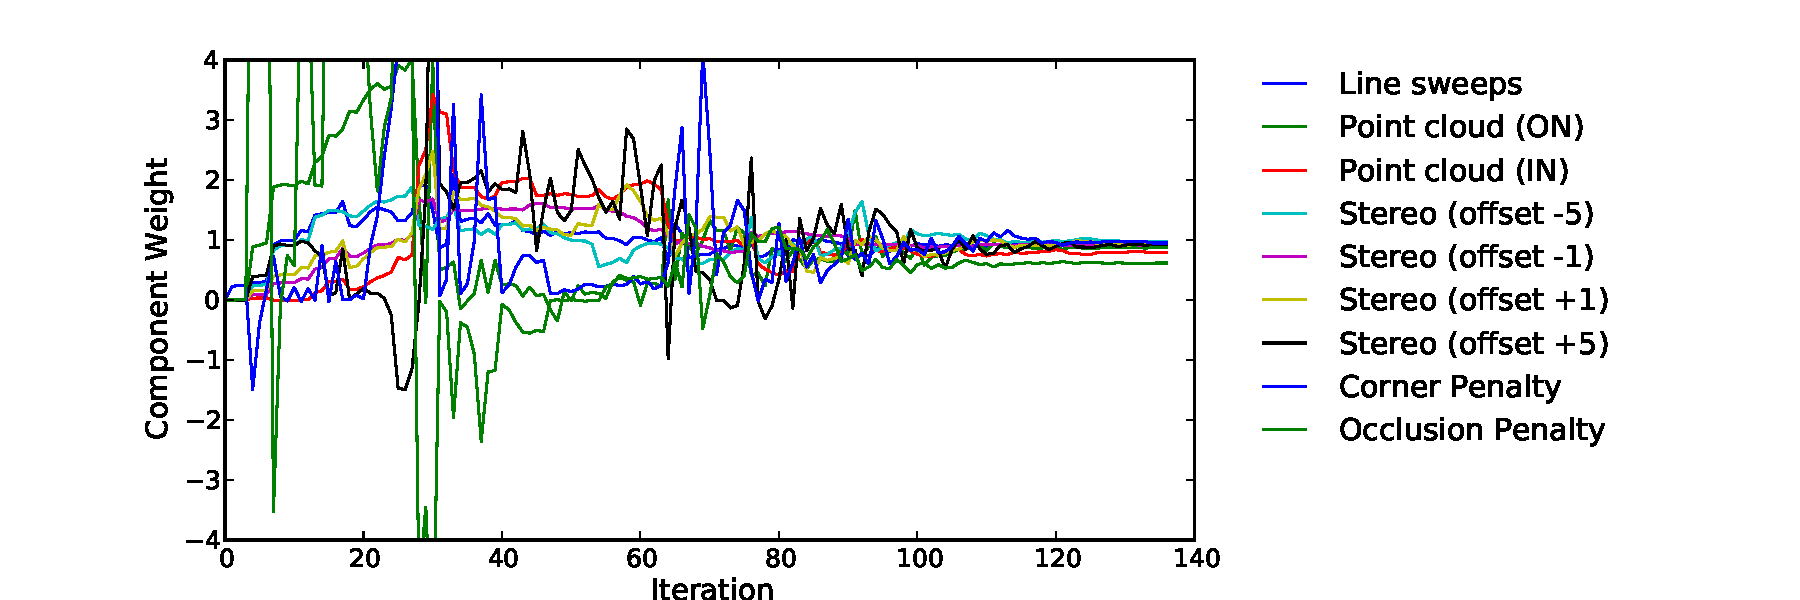
\includegraphics[width=\textwidth]{psi_evolution_mview_depth}
  }
  \\
  \subfloat[Evolution of $\Fmviewlbl$ during training]{
    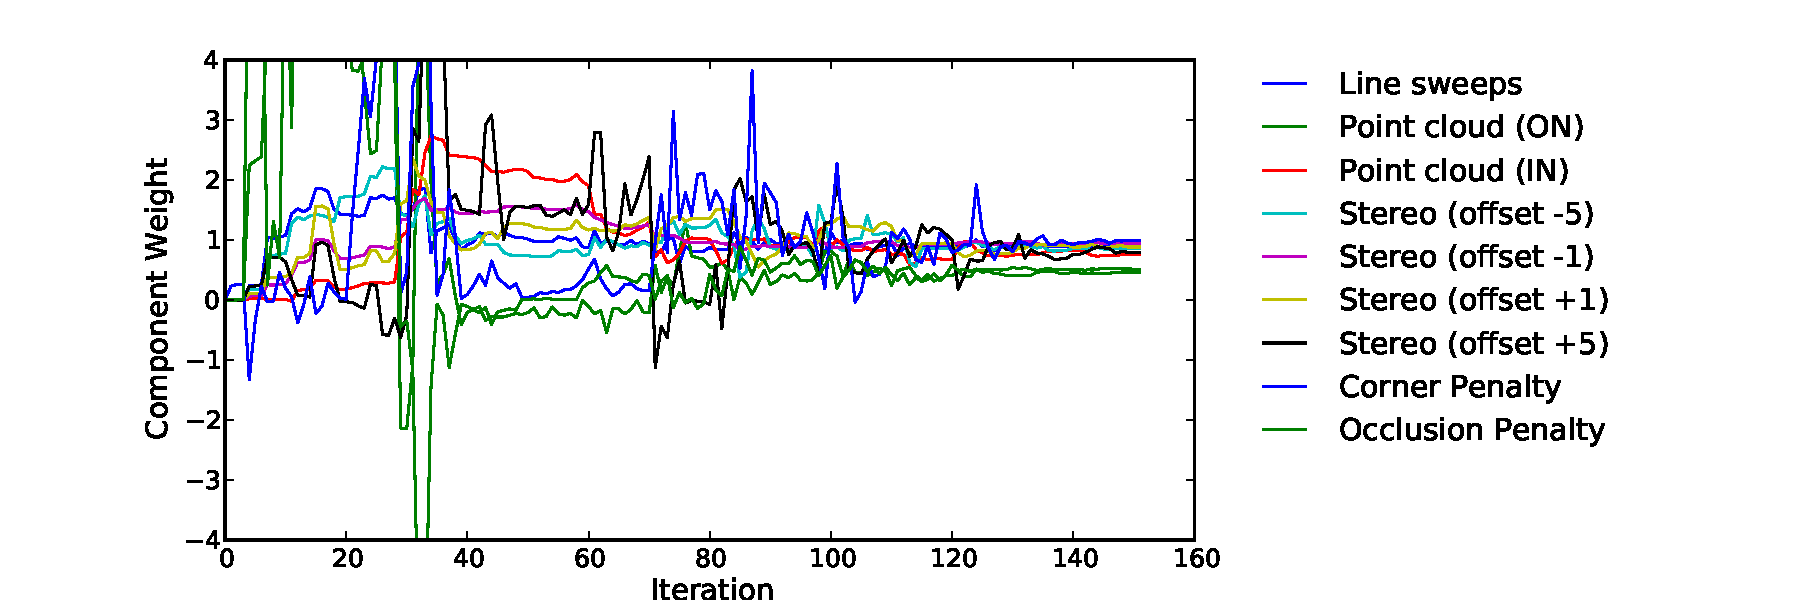
\includegraphics[width=\textwidth]{psi_evolution_mview_lbl}
  }
  \\
  \subfloat[Evolution of $\Fsviewdepth$ during training (selected
    features only)]{
    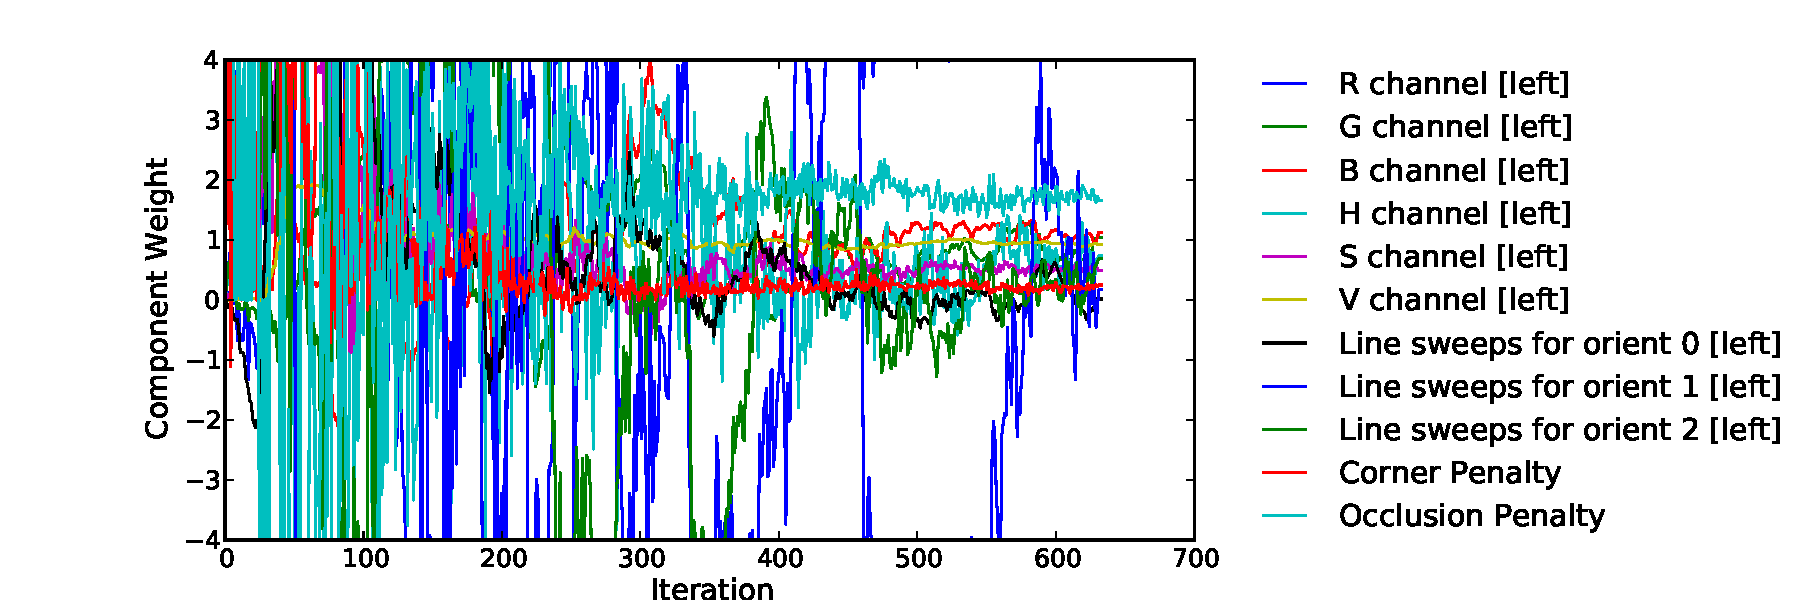
\includegraphics[width=\textwidth]{psi_evolution_sview_depth}
  }
  \\
  \subfloat[Evolution of $\Fsviewlbl$ during training (selected
    features only)]{
    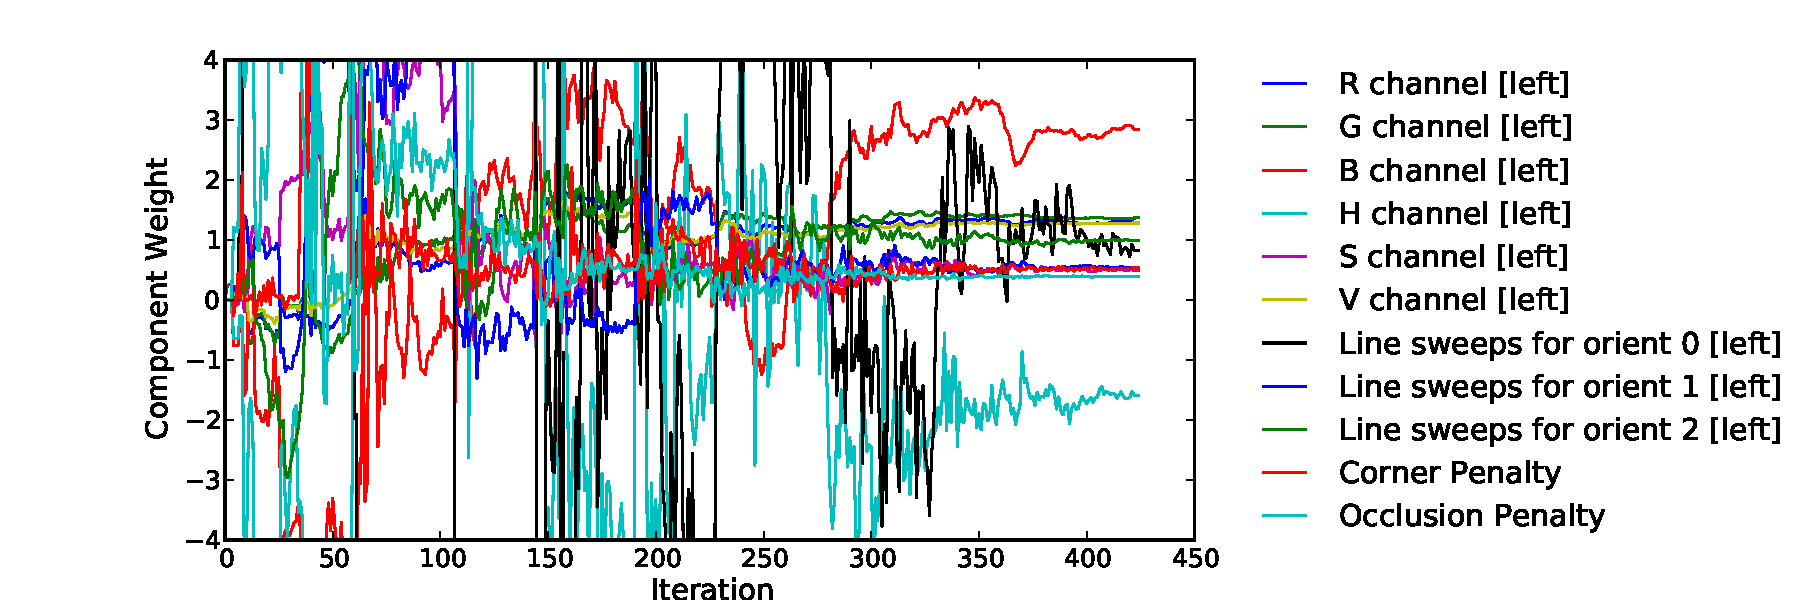
\includegraphics[width=\textwidth]{psi_evolution_sview_lbl}
  }
  \caption{Evolution of weights during training of each predictor.}
  \label{fig:psi-evolution}
\end{figure}

In the main paper we reported performance for each predictor on
held--out training data. We reported only the performance metric
corresponding to the loss for which each predictor was trained. Here
we report performance for both metrics, for all predictors. That is,
for each predictor, we compute both the depth and labelling error,
regardless of which loss the predictor was trained against. These
results are summarized in \figref{performance}.

Finally we show examples of predictions made by our system and the
comparison systems in Tables 1 and 2.

\begin{figure}[h]
  \centering

\subfloat[Relative depth error]{
  \begin{tabular}{@{}p{20mm}rrrrrr@{}}
    \toprule
      Sequence & 
      $\Fmviewdepth$ &
      \hspace{3mm} $\Fmviewlbl$ &
      \hspace{6mm} \cite{Flint11} &
      \hspace{3mm} $\Fsviewdepth$ &
      \hspace{3mm} $\Fsviewlbl$ &
      \hspace{6mm} \cite{Flint10eccv} \\
    \midrule
      \tt{ground}     &   4.9 &   5.5 &  66.6 &  17.3 &  28.0 &  24.5 \\
      \tt{foyer1}     &   6.1 &   4.5 &   6.6 &  25.1 &  29.2 &  31.0 \\
      \tt{foyer2}     &   4.3 &   4.9 &   5.4 &  29.1 &  28.5 &  30.1 \\
      \tt{corridor}   &  14.6 &  15.0 &  52.9 &  31.7 &  32.7 &  33.6 \\
      \tt{mcr}        &  34.0 &  37.3 &  67.6 &  70.1 &  58.6 &  45.9 \\
      \tt{kitchen}    &  16.8 &  19.3 &  23.6 &  25.1 &  25.8 &  26.2 \\
    \midrule
      Average         &  \textbf{13.4} &  14.4 &  37.1 &  33.1 &  33.8 &  31.9 \\
    \bottomrule
  \end{tabular}
}
\\
\subfloat[Labelling error]{
  \begin{tabular}{@{}p{20mm}rrrrrr@{}}
    \toprule
      Sequence & 
      $\Fmviewdepth$ &
      \hspace{3mm} $\Fmviewlbl$ &
      \hspace{6mm} \cite{Flint11} &
      \hspace{3mm} $\Fsviewdepth$ &
      \hspace{3mm} $\Fsviewlbl$ &
      \hspace{6mm} \cite{Flint10eccv} \\
    \midrule
      \tt{ground}     &   2.8 &   2.9 &  10.4 &  14.8 &   7.8 &  12.4 \\
      \tt{foyer1}     &   3.6 &   3.1 &   3.1 &  20.3 &  15.1 &  22.2 \\
      \tt{foyer2}     &   3.3 &   3.7 &   4.0 &  18.6 &  15.9 &  18.6 \\
      \tt{corridor}   &  11.4 &   9.5 &  19.2 &  23.7 &  19.3 &  24.8 \\
      \tt{mcr}        &  15.4 &  15.8 &  16.2 &  24.5 &  26.7 &  20.8 \\
      \tt{kitchen}    &   5.3 &   5.2 &   6.1 &  11.0 &   7.7 &  11.9 \\
    \midrule
      Average         &   7.0 &   \textbf{6.7} &   9.8 &  18.8 &  15.4 &  18.4 \\
    \bottomrule
  \end{tabular}
}

\caption{Performance for each predictor, for each sequence, and for
  each error metric. The six predictors under comparison are listed in
  the top row of each table. Note that even when a predictor is
  trained with respect to a particular loss function, we may still
  evaluate it on hold--out data using a different metric. However, as
  exepected the predictors perform best when evaluated by the same
  error metric that they were each trained for.}
  \label{fig:performance}
\end{figure}


\subsection{Examples of outputs from our system}

\newcommand{\CompFrame}[3]{
  \includegraphics[width=0.18\textwidth]
                  {figures_addendum/examples/#1_frame#2_#3.jpg}
}

\newcommand{\MviewRow}[2]{
  \CompFrame{#1}{#2}{mview_depth} &
  \CompFrame{#1}{#2}{mview_lbl} &
  \CompFrame{#1}{#2}{iccv} &
  \CompFrame{#1}{#2}{gt}
}

\newcommand{\SviewRow}[2]{
  \CompFrame{#1}{#2}{sview_depth} &
  \CompFrame{#1}{#2}{sview_lbl} &
  \CompFrame{#1}{#2}{eccv} &
  \CompFrame{#1}{#2}{gt}
}

\begin{centering}
  \begin{longtable}{cccc}
    \caption{Reconstructions predicted by our system using the
      multiple view feature space; comparison with Flint \etal
      \cite{Flint11}. Instances in this figure are samples from the
      hold--out set.
    }\\

    $\Fmviewdepth$ & $\Fmviewdepth$ & Flint \etal \cite{Flint11} & Ground Truth \\
    \endfirsthead

    $\Fmviewdepth$ & $\Fmviewdepth$ & Flint \etal \cite{Flint11} & Ground Truth \\
    \endhead

    \multicolumn{4}{r}{Continued on next page} \\
    \endfoot
    \endlastfoot

    \MviewRow{lab_kitchen1}{002} \\
    \MviewRow{lab_kitchen1}{012} \\
    \MviewRow{lab_kitchen1}{022} \\
    \MviewRow{lab_kitchen1}{032} \\
    \MviewRow{lab_kitchen1}{042} \\
    \MviewRow{lab_kitchen1}{052} \\
    \MviewRow{lab_kitchen1}{062} \\
    \MviewRow{lab_kitchen1}{072} \\
    \MviewRow{lab_kitchen1}{082} \\
    \MviewRow{lab_kitchen1}{092} \\

    \MviewRow{exeter_mcr1}{002} \\
    \MviewRow{exeter_mcr1}{012} \\
    \MviewRow{exeter_mcr1}{022} \\
    \MviewRow{exeter_mcr1}{032} \\
    \MviewRow{exeter_mcr1}{042} \\
    \MviewRow{exeter_mcr1}{052} \\

    \MviewRow{lab_foyer1}{002} \\
    \MviewRow{lab_foyer1}{012} \\
    \MviewRow{lab_foyer1}{022} \\
    \MviewRow{lab_foyer1}{032} \\
    \MviewRow{lab_foyer1}{042} \\

    \MviewRow{lab_foyer2}{002} \\
    \MviewRow{lab_foyer2}{012} \\
    \MviewRow{lab_foyer2}{022} \\
    \MviewRow{lab_foyer2}{032} \\
    \MviewRow{lab_foyer2}{042} \\

    \MviewRow{som_corr1}{012} \\
    \MviewRow{som_corr1}{022} \\
    \MviewRow{som_corr1}{032} \\
    \MviewRow{som_corr1}{042} \\

    \MviewRow{lab_ground1}{002} \\
    \MviewRow{lab_ground1}{012} \\
    \MviewRow{lab_ground1}{022} \\
    \MviewRow{lab_ground1}{032} \\
    \MviewRow{lab_ground1}{042} \\
  \end{longtable}
\end{centering}


\begin{centering}
  \begin{longtable}{cccc}
    \caption{Reconstructions predicted by our system using the single
      view feature space; comparison with Flint \etal
      \cite{Flint11}. Instances in this figure are samples from the
      hold--out set.}\\

    $\Fmviewdepth$ & $\Fmviewdepth$ & Flint \etal \cite{Flint10eccv} & Ground Truth \\
    \endfirsthead

    $\Fmviewdepth$ & $\Fmviewdepth$ & Flint \etal \cite{Flint10eccv} & Ground Truth \\
    \endhead

    \multicolumn{4}{r}{Continued on next page} \\
    \endfoot
    \endlastfoot

    \SviewRow{lab_kitchen1}{002} \\
    \SviewRow{lab_kitchen1}{012} \\
    \SviewRow{lab_kitchen1}{022} \\
    \SviewRow{lab_kitchen1}{032} \\
    \SviewRow{lab_kitchen1}{042} \\
    \SviewRow{lab_kitchen1}{052} \\
    \SviewRow{lab_kitchen1}{062} \\
    \SviewRow{lab_kitchen1}{072} \\
    \SviewRow{lab_kitchen1}{082} \\
    \SviewRow{lab_kitchen1}{092} \\

    \SviewRow{exeter_mcr1}{002} \\
    \SviewRow{exeter_mcr1}{012} \\
    \SviewRow{exeter_mcr1}{022} \\
    \SviewRow{exeter_mcr1}{032} \\
    \SviewRow{exeter_mcr1}{042} \\
    \SviewRow{exeter_mcr1}{052} \\

    \SviewRow{lab_foyer1}{002} \\
    \SviewRow{lab_foyer1}{012} \\
    \SviewRow{lab_foyer1}{022} \\
    \SviewRow{lab_foyer1}{032} \\
    \SviewRow{lab_foyer1}{042} \\

    \SviewRow{lab_foyer2}{002} \\
    \SviewRow{lab_foyer2}{012} \\
    \SviewRow{lab_foyer2}{022} \\
    \SviewRow{lab_foyer2}{032} \\
    \SviewRow{lab_foyer2}{042} \\

    \SviewRow{som_corr1}{012} \\
    \SviewRow{som_corr1}{022} \\
    \SviewRow{som_corr1}{032} \\
    \SviewRow{som_corr1}{042} \\

    \SviewRow{lab_ground1}{002} \\
    \SviewRow{lab_ground1}{012} \\
    \SviewRow{lab_ground1}{022} \\
    \SviewRow{lab_ground1}{032} \\
    \SviewRow{lab_ground1}{042} \\
  \end{longtable}
\end{centering}

\bibliographystyle{splncs}
\bibliography{AVLstrings,VisionRefs,MendeleyRefs}


\end{document}
